\documentclass[12pt,norsk,a4paper]{article}
\usepackage{setspace}
\usepackage{color}
\usepackage{listings}
\definecolor{mygreen}{rgb}{0,0.6,0}
\definecolor{mygray}{rgb}{0.5,0.5,0.5}
\definecolor{mymauve}{rgb}{0.58,0,0.82}
\usepackage{graphicx}
\usepackage[english]{babel}
\usepackage[latin1]{inputenc}
\usepackage[T1]{fontenc}
\lstset{ %
  backgroundcolor=\color{white},   % choose the background color; you must add \usepackage{color} or \usepackage{xcolor}
  basicstyle=\footnotesize,        % the size of the fonts that are used for the code
  breakatwhitespace=false,         % sets if automatic breaks should only happen at whitespace
  breaklines=true,                 % sets automatic line breaking
  captionpos=b,                    % sets the caption-position to bottom
  commentstyle=\color{mygreen},    % comment style
  deletekeywords={...},            % if you want to delete keywords from the given language
  escapeinside={\%*}{*)},          % if you want to add LaTeX within your code
  extendedchars=true,              % lets you use non-ASCII characters; for 8-bits encodings only, does not work with UTF-8
  frame=single,                    % adds a frame around the code
  keepspaces=true,                 % keeps spaces in text, useful for keeping indentation of code (possibly needs columns=flexible)
  keywordstyle=\color{blue},       % keyword style
  language=Python,                 % the language of the code
  morekeywords={*,...},            % if you want to add more keywords to the set
  numbers=none,                    % where to put the line-numbers; possible values are (none, left, right)
  numbersep=5pt,                   % how far the line-numbers are from the code
  numberstyle=\tiny\color{mygray}, % the style that is used for the line-numbers
  rulecolor=\color{black},         % if not set, the frame-color may be changed on line-breaks within not-black text (e.g. comments (green here))
  showspaces=false,                % show spaces everywhere adding particular underscores; it overrides 'showstringspaces'
  showstringspaces=false,          % underline spaces within strings only
  showtabs=false,                  % show tabs within strings adding particular underscores
  stepnumber=2,                    % the step between two line-numbers. If it's 1, each line will be numbered
  stringstyle=\color{mymauve},     % string literal style
  tabsize=2,                       % sets default tabsize to 2 spaces
  title=\lstname                   % show the filename of files included with \lstinputlisting; also try caption instead of title
}

\begin{document}
\begin{titlepage}
\begin{center}
AST1100\\
Oblig11\\
Lecture 17 - Problem 2\\
-\\
Thor Andreas Seiff Ellewsen\\
tellewsen@gmail.com\\
\end{center}
The assignment this week is to model the path of a spaceships towards a black hole. This is done using the geometry of spacetime instead of forces. There's not much to explain this week since the assignment is done step by step through the exercise. All the values used are either given in the text or taken from the solution for the last exercise. This means that pretty much all there is to show for this week is the python code I made. There are comments in the code which explain what each section of code does.\\
\\
Here's a quick explanation of the problem:\\
We are to start the spaceship at a distance $r=20M$ from the blackhole with an angle $phi = 0$.
We then evolve the position of the ship using equations 2 and 3 from the lecture notes.
The only question that we get is what the final angle of the ship is.
The answer to that can be read in the part with the output of the program in the end.
\end{titlepage}

\lstinputlisting[language=Python]{oblig11.py}
After the code is run we get the following output:\\
Final phi:  202.784147091\\

\begin{figure}[h]
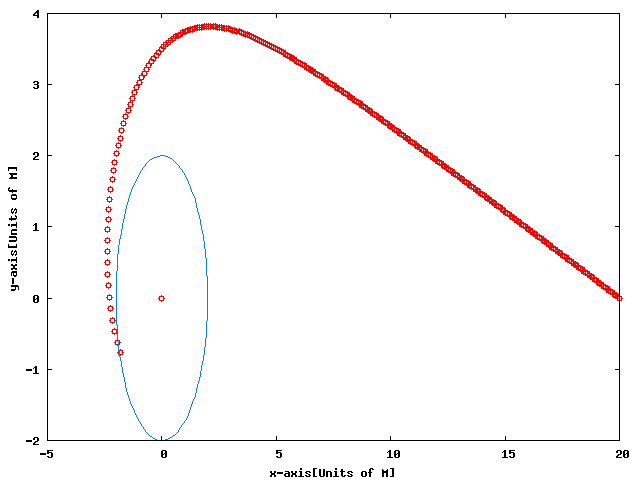
\includegraphics[width=\textwidth]{oblig11.png}
\caption{Path of the spaceship}
\end{figure}

\newpage
Conclusion:\\
The final angle corresponds to the point where the spaceship enters the event horizon on the plot. This is as expected.\\ 
The spaceship starts out going in the direction it did in the first exercise. This is as expected.\\
The path looks like the path gravity would force the spaceship to go so I guess I've done this right.\\
\end{document}